\documentclass[11  pt]{article} 
\usepackage[lmargin=1in,rmargin=1.75in,bmargin=1in,tmargin=1in]{geometry}  


% For hyperlinking everything
\usepackage{hyperref}
\hypersetup{
	colorlinks=true, %set true if you want colored links
	linktoc=all,     %set to all if you want both sections and subsections linked
	linkcolor=blue,  %choose some color if you want links to stand out
}


\usepackage[latin1]{inputenc}
\usepackage{amsmath}
\usepackage{mathrsfs}  
\usepackage{amsfonts}
\usepackage{amssymb}
\usepackage{graphicx}
\usepackage{subfig}
\usepackage{caption}
\usepackage{algorithm}
%\usepackage{algcompatible}
%\usepackage{algorithmicx}
\usepackage{algpseudocode}

\usepackage{titlesec}
\titleformat{\section}{\fontfamily{lmss}\fontsize{14}{15}\bfseries}{\thesection}{1em}{}
\titleformat{\subsection}{\fontfamily{lmss}\fontsize{12}{15}\bfseries}{\thesubsection}{1em}{}




\usepackage{amsthm}

\newtheoremstyle{noit}
{10pt}% <Space above>
{10pt}% <Space below>
{}% <Body font>
{}% <Indent amount>
{\bfseries}% <Theorem head font>
{.}% <Punctuation after theorem head>
{.5em}% <Space after theorem headi>
{}% <Theorem head spec (can be left empty, meaning `normal')>

\newtheoremstyle{example}
{10pt}% <Space above>
{10pt}% <Space below>
{}% <Body font>
{20pt}% <Indent amount>
{\bfseries}% <Theorem head font>
{.}% <Punctuation after theorem head>
{.5em}% <Space after theorem headi>
{}% <Theorem head spec (can be left empty, meaning `normal')>


\newtheoremstyle{indented}{20pt}{20pt}{\addtolength{\leftskip}{2.5em}}{}{\bfseries}{.}{.5em}{}


\newtheorem{theorem}{Theorem}
\numberwithin{theorem}{section}
\newtheorem{lemma}[theorem]{Lemma}
\newtheorem{corollary}[theorem]{Corollary}
\newtheorem{observation}{Observation}
%\numberwithin{observation}{section}
%\numberwithin{definition}{section}
\newtheorem{conjecture}{Conjecture}
\newtheorem{Qu}{Question}
\newcommand{\QU}{\begin{Qu}\normalfont}

\theoremstyle{noit}
\newtheorem{fact}{Fact}
\newtheorem{definition}{Definition}

\theoremstyle{indented}
\newtheorem{example}{Example}

\theoremstyle{indented}
\newtheorem{problem}{Problem}


%\newenvironment{proof}{\noindent{\bf Proof:} \hspace*{1em}}{
%    \hspace*{\fill} $\Box$ }
%\newenvironment{proof_of}[1]{\noindent {\bf Proof of #1:}
%    \hspace*{1em} }{\hspace*{\fill} $\Box$ }
%\newenvironment{proof_claim}{\begin{quotation} \noindent}{
%    \hspace*{\fill} $\diamond$ \end{quotation}}
\newcommand{\vs}[1]{\vspace{#1}}

\newcommand{\lecture}[2]{
 \noindent
\begin{center}
	\framebox{
		\vbox{
			\hbox to 5.78in { {\bf CSCE 411: Design and Analysis of Algorithms} \hfill  }
			\vspace{2mm}
			\hbox to 5.78in { {\Large \hfill Lecture #1\hfill} }
			\vspace{2mm}
			\hbox to 5.78in { {\it Date: #2 \hfill Lecturer: Nate Veldt} }
		}
	}
\end{center}
\vspace*{4mm}
}


\newcommand{\hw}[2]{
	\noindent
	\begin{center}
		\framebox{
			\vbox{
				\hbox to 5.78in { {\bf CSCE 411: Design and Analysis of Algorithms} \hfill  }
				\vspace{2mm}
				\hbox to 5.78in { {\Large \hfill Homework #1\hfill} }
				\vspace{2mm}
				\hbox to 5.78in { {\it Due date: #2 \hfil} }
			}
		}
	\end{center}
	\vspace*{4mm}
}



\newcommand{\under}[1]{\underline{\hspace{#1}}}
\setlength{\parindent}{0em}

%\usepackage[tagged]{accessibility}

% Graph terms
\newcommand{\vol}{\textbf{vol}}
\newcommand{\cut}{\textbf{cut}}


% Matrices
\newcommand{\mA}{\textbf{A}}
\newcommand{\mB}{\textbf{B}}

% vectors
\newcommand{\ve}{\textbf{e}}
\newcommand{\vx}{\textbf{x}}


% Other
\newcommand{\calN}{\mathcal{N}}

\usepackage{mathtools}
\DeclarePairedDelimiter\ceil{\lceil}{\rceil}
\DeclarePairedDelimiter\floor{\lfloor}{\rfloor}


\newcommand*{\aitem}{ \item[{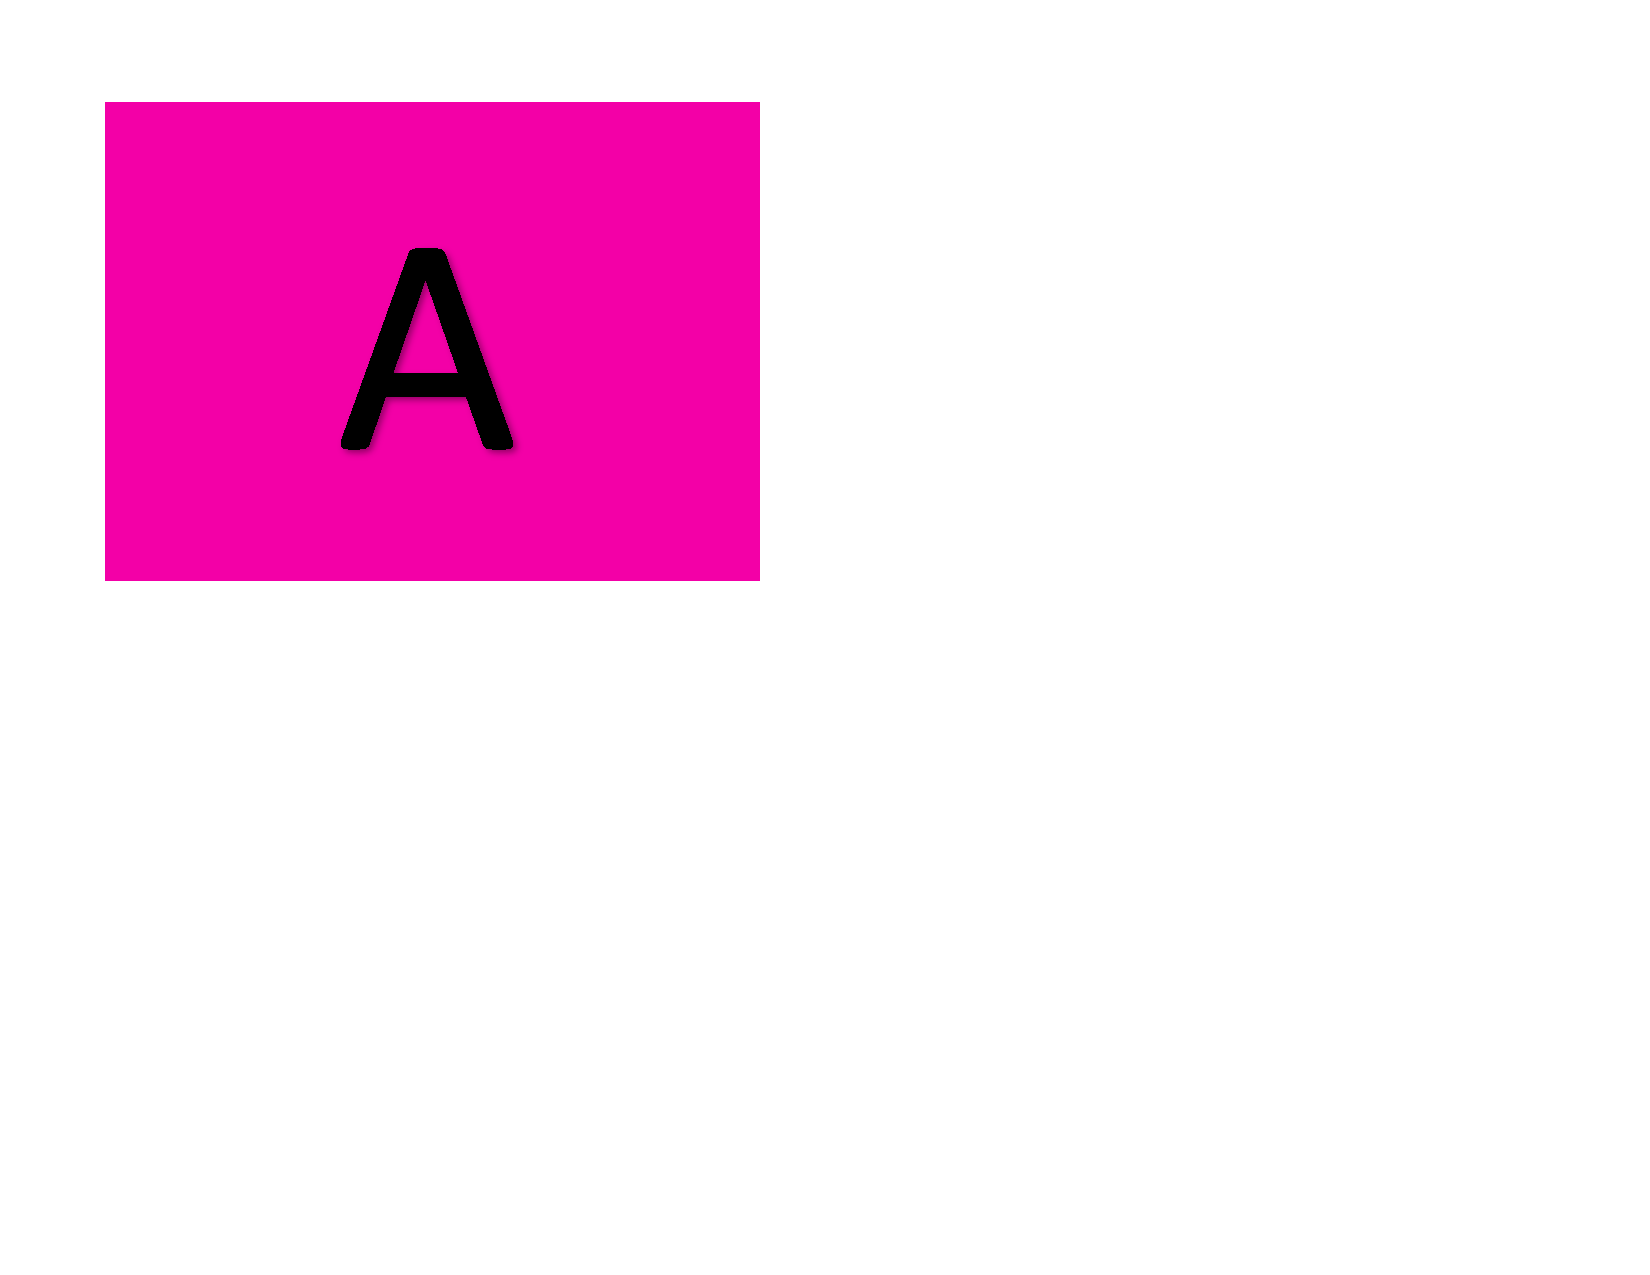
\includegraphics[width=0.8cm,height=0.5cm]{../../Lectures/figures/A}} ]  }
\newcommand*{\bitem}{ \item[{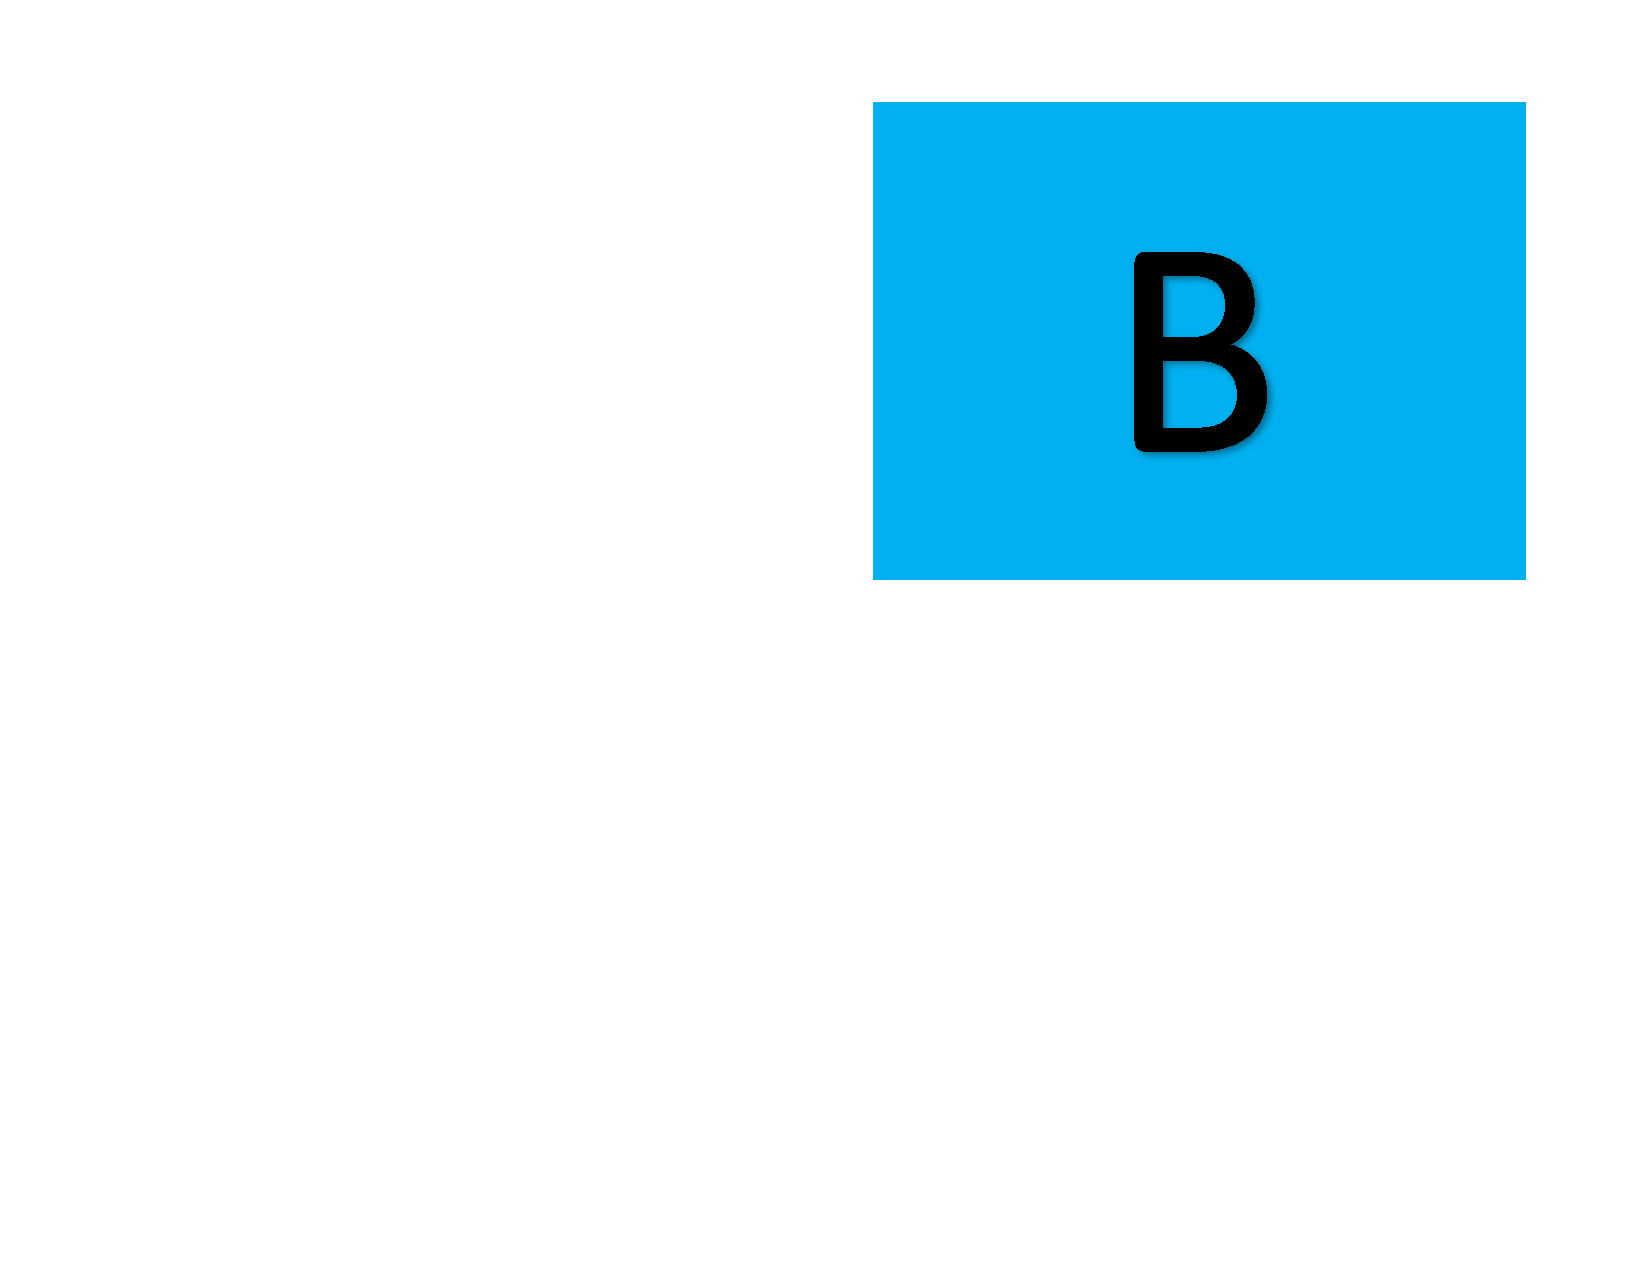
\includegraphics[width=0.8cm,height=0.5cm]{../../Lectures/figures/B}} ]  }
\newcommand*{\citem}{ \item[{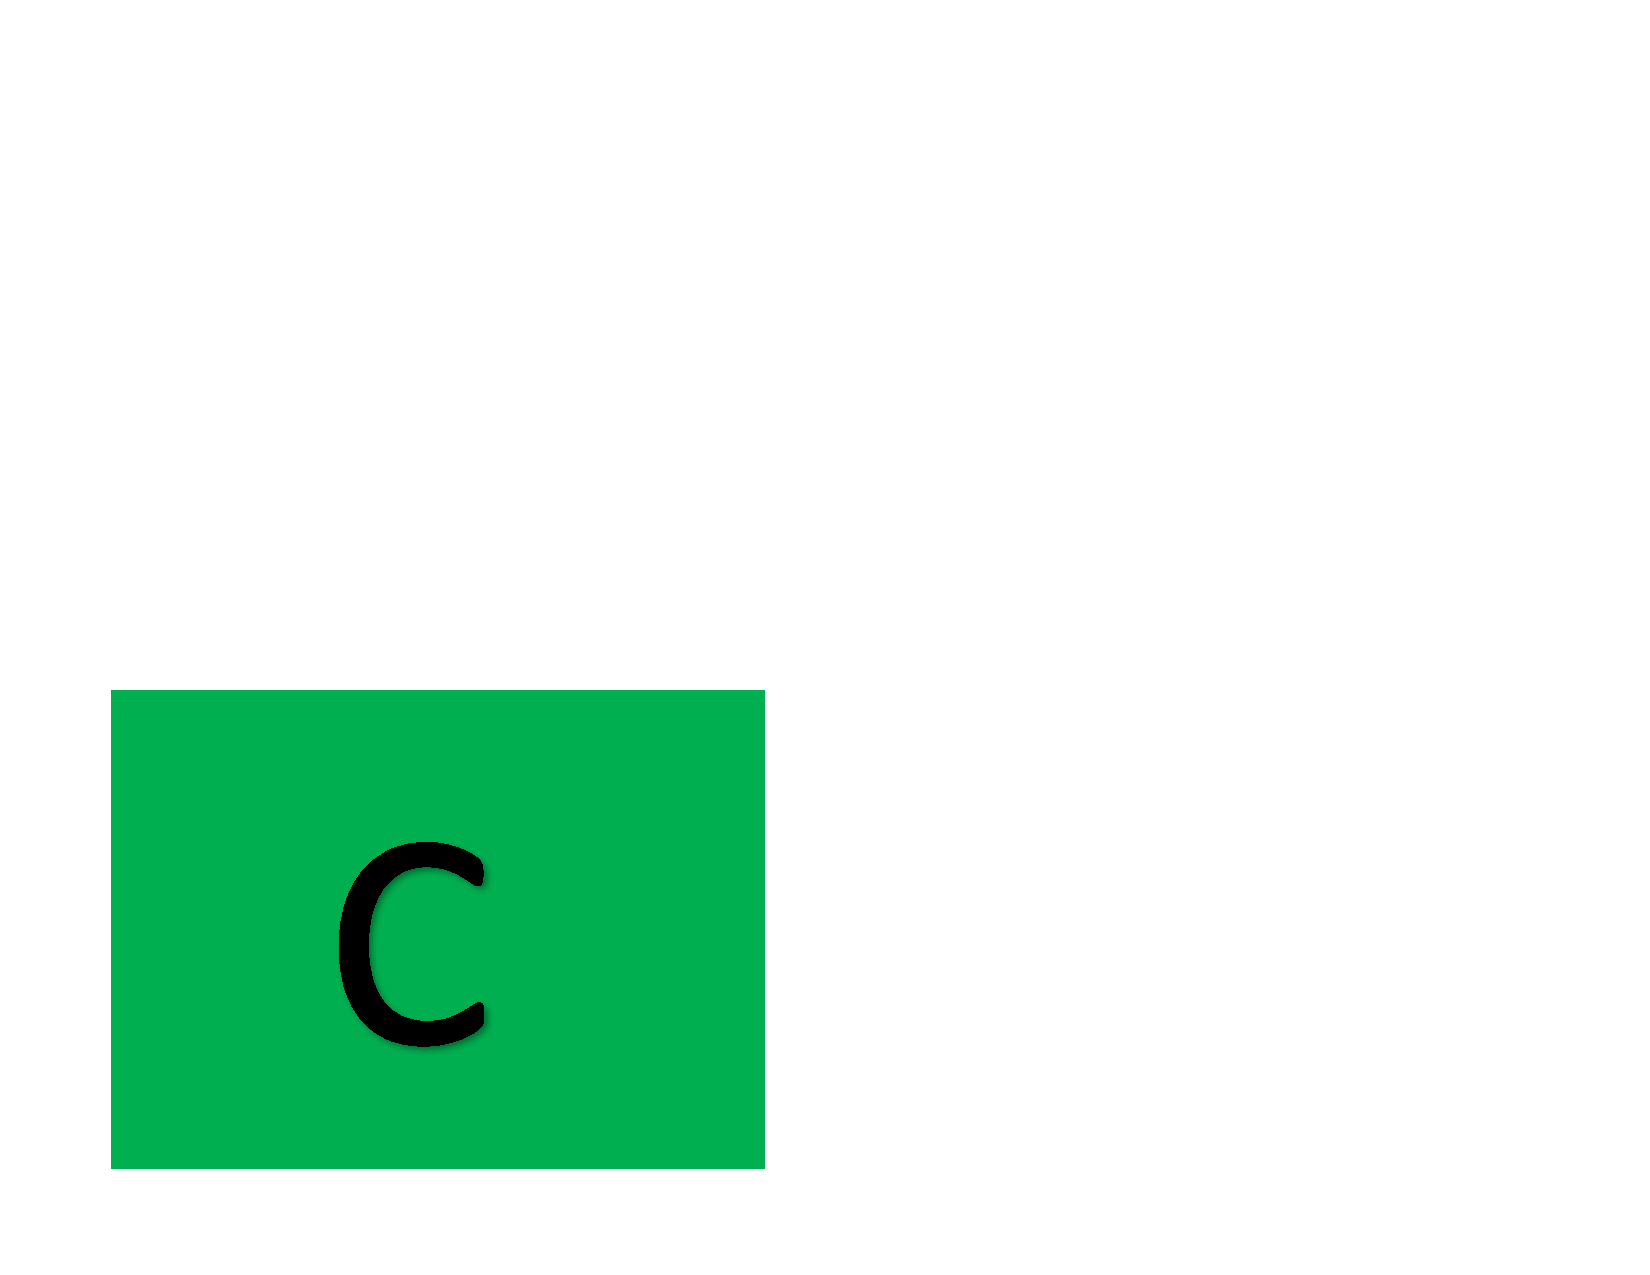
\includegraphics[width=0.8cm,height=0.5cm]{../../Lectures/figures/C}} ]  }
\newcommand*{\ditem}{ \item[{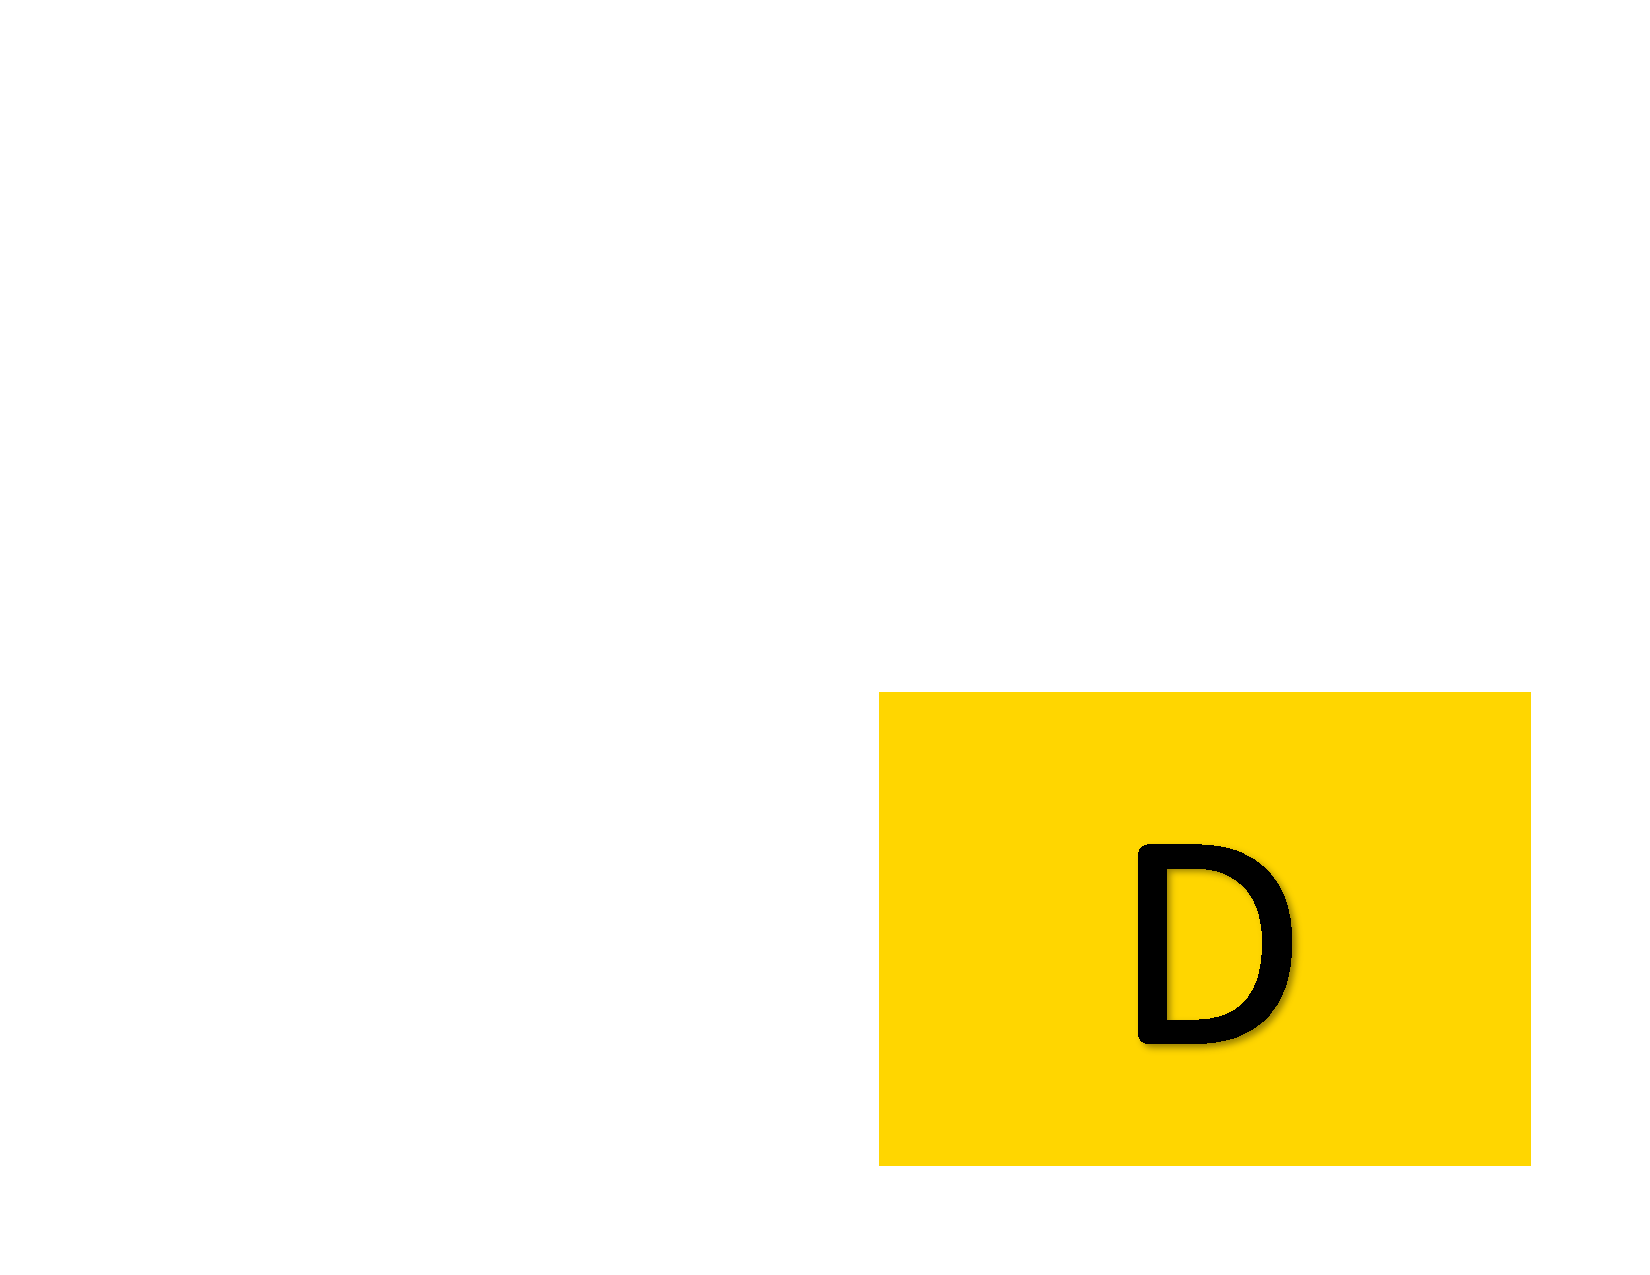
\includegraphics[width=0.8cm,height=0.5cm]{../../Lectures/figures/D}} ]  }
\newcommand*{\eitem}{ \item[{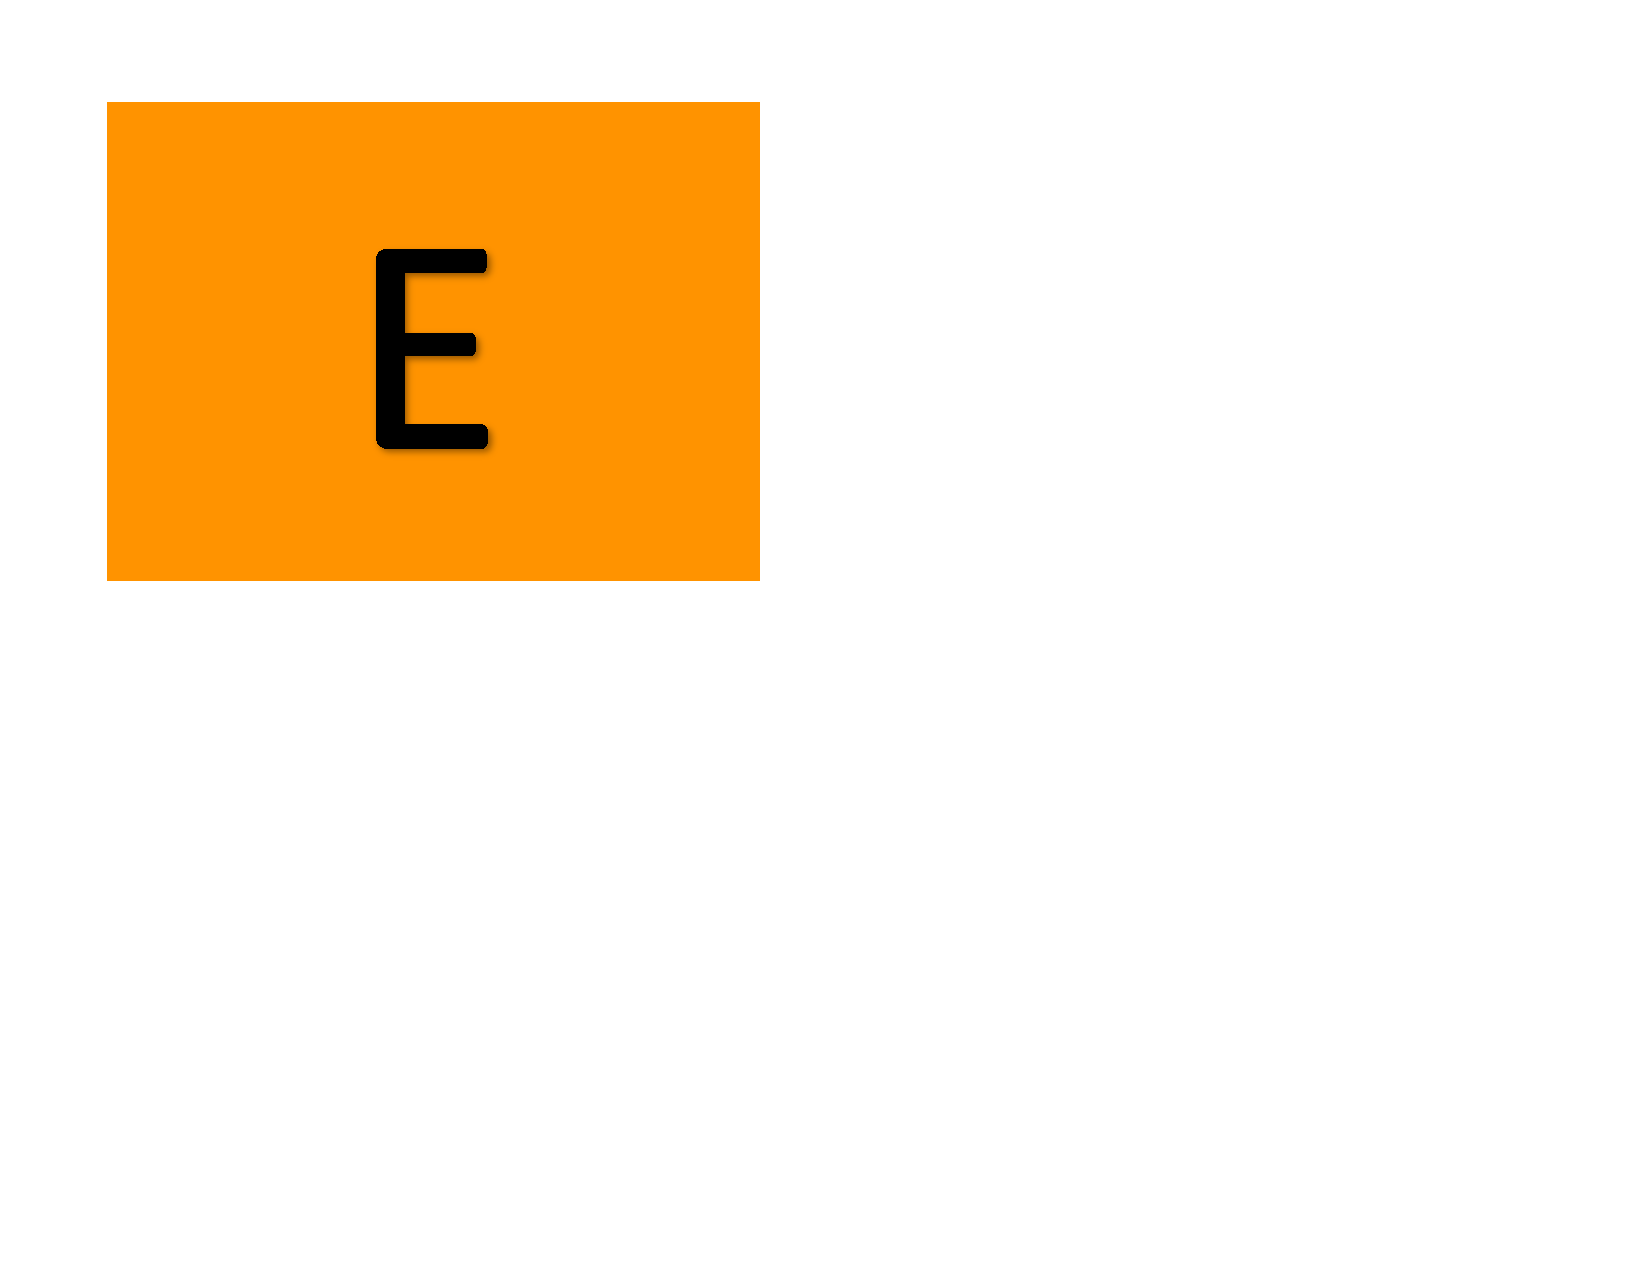
\includegraphics[width=0.8cm,height=0.5cm]{../../Lectures/figures/E}} ]  }
\newcommand*{\fitem}{ \item[{
\includegraphics[width=0.8cm,height=0.5cm]{../../Lectures/figures/F}} ]  }


\newcommand{\hide}[1]{\underline{\phantom{#1 #1}}}

\usepackage{setspace}

\onehalfspacing

\begin{document}
	
	
	\lecture{3: Dynamic Programming: First Week}{January 23, 2025}
	
	\paragraph{Course Logistics}
	
	\begin{itemize}
		\item Read chapter 15 over the course of the next few lectures (focus: 15.1, 15.2, 15.3).
		\item Homework 1 and intro video due this Friday (tomorrow)
	\end{itemize}
	
	\paragraph{Intro Poll}
	
	\QU
	The Fibonacci sequence is given by:
	\begin{align*}
		F_0 &= 0 \\
		F_1 &= 1 \\
		F_n &= F_{n-1} + F_{n-2} \text{ for $n > 1$}
	\end{align*}
	What is $F_8$?
	\begin{enumerate}
		\aitem 6
		\bitem 8
		\citem 13
		\ditem 21
		\eitem 377
	\end{enumerate}
\end{Qu}

\newpage
\section{Dynamic Programming}

Dynamic Programming breaks down a larger problem into smaller subproblems, similar to \hide{Divide-and-Conquer.} \\

This paradigm is often used specifically for \hide{\textbf{optimization}} problems. \\

Dynamic Programming is designed for problems that satisfy two properties:
\begin{itemize}
	\item \textbf{Optimal substructure}: %an optimal solution to the problem contains optimal solutions to smaller problems
	\vs{2cm}
	
	\item \textbf{Overlapping subproblems}:% many of the smaller problems are repeats of the same problem \\
\end{itemize}
\vs{2cm}

\QU
Which property is also satisfied by the Divide-and-Conquer approach?
\begin{enumerate}
	\aitem Optimal substructure
	\bitem Overlapping subproblems
	\citem Both of the above
	\ditem None of the above
\end{enumerate}
\end{Qu}
\newpage

\paragraph{Class activity: Fibonacci sequence}
The Fibonacci sequence is given by:
\begin{align*}
F_0 &= 0 \\
F_1 &= 1 \\
F_n &= F_{n-1} + F_{n-2} \text{ for $n > 1$}
\end{align*}
Here's a naive algorithm that works for computing $F_k$.
\begin{algorithm}
\textsc{Fib}(n)
\begin{algorithmic}
	\If{$n == 0$}
	\State Return 0
	\ElsIf{$n == 1$}
	\State Return 1
	\Else
	\State Return $\textsc{Fib}(n-1) + \textsc{Fib}(n-2)$
	\EndIf
\end{algorithmic}
\end{algorithm}

\emph{Some questions}
\begin{enumerate}
\item How does this problem satisfy the two conditions for dynamic programming?

\item What's wrong or inefficient about the Fibonacci sequence? (Try using it to compute $F_4$ or $F_5$.)

\item What's a strategy for fixing the inefficiency?
\end{enumerate}


\newpage
\section{The Rod Cutting Problem}
Let $p_i$ equal the \hide{price for buying $i$ inches of steel rod.}

\begin{problem}(The Rod Cutting Problem.)
Given a rod of length $n$ inches, determine how to cut it into pieces to:

%maximize the sum of costs for the subpieces. 
\vs{2cm}

All subpieces have an integer length in inches.
\end{problem}

\paragraph{Try a few small values of $i$}
We can set up a price table, and let $r_i = $ optimal cost for a rod of size $i$.\\

{\Huge
\begin{center}
	\begin{tabular}{c | c | c | c | c | c | c | c | c | c | c }
		$i$ & 1 & 2 & 3 & 4 & 5 & 6 & 7 & 8 & 9 & 10 \\
		\hline
		$p_i$ & 1 & 5 & 8 & 9 & 10 & 17 & 17 & 20 & 24 & 30  \\
		\hline
		$r_i$ &  & & & & & & & & & 
	\end{tabular} \\
\end{center}
}

\newpage
\paragraph{Generalizing our strategy}

\vs{2cm}

\begin{theorem}
The problem satisfies the following structure:

\vs{2cm}

Meaning: the optimal solution for $n$ is the same as finding the best way to split it into two pieces, and then split these sub-rods in their optimal ways.
\end{theorem}

\vs{4cm}

Why? \\ \\%If you cut a length $n$ rod into pieces of length $k$ and $n-k$ but don't use the optimal way to cut these sub-rods, you can always instead go back and use the optimal cuts for these sub-robs to get a better solution.
\vs{3cm}

\begin{theorem}
The problem satisfies the following even simpler characterization:
\vs{3cm}
\end{theorem}
Why?

\newpage

\subsection{Runtime Analysis for a Bottom-Up Approach}

\vs{1cm}
{\Large
%\begin{align*}
$r_0 = 0$ \\ \\
$r_1 = p_1 $\\\\
$r_2 = \max \{ p_1 + r_1, p_2 + r_0\} $\\\\
$r_3 = \max \{ p_1 + r_2, p_2 + r_1, p_3 + r_0\}$ \\\\
$\vdots $\\\\
$r_n = \max \{ p_1 + r_{n-1}, p_2 + r_{n-2}, \hdots , p_n + r_0\} $\\
}%\end{align*}




\newpage

\section{The Longest Common Subsequence Problem}

\paragraph{Preliminaries} A sequence is an ordered list of elements:\\
\begin{equation*}
	X = \langle x_1, x_2, \hdots ,x_m \rangle
\end{equation*}

A subsequence of $X$ is a sequence you obtain by deleting elements of $X$. \\

A sequence $Z = \langle z_1, z_2, \hdots , z_k \rangle$ is a subsequence of $X$ if there are indices $i_1 < i_2 < \cdots < i_k$ such that:
\begin{equation*}
	z_1 = x_{i_1}, z_2 = x_{i_2}, \hdots, z_k = x_{i_k}.
\end{equation*}

\paragraph{Example}


\newpage

\subsection{Defining the LCS Problem}
Given two sequences 
\begin{align*}
	X = \langle x_1, x_2, \hdots ,x_m \rangle \\
	Y = \langle y_1, y_2, \hdots ,y_n \rangle
\end{align*}
A \emph{longest common subsequence} (LCS) of $(X,Y)$ is a \\

%	seeks a maximum length-sequence $Z = \langle z_1, z_2, \hdots , z_k \rangle$ that is a subsequence of both $X$ and $Y$.

\vs{1cm}

%\QU 
%A brute force algorithm for the LCS problem would be to consider every subsequence of $X$ and check if it's a subsequence of $Y$. Define:
%\begin{center}
%	$N = $ be the number of subsequences of $X$,
%\end{center} and let $T$ be the time it takes to check whether a sequence $Z$ is a subsequence of $Y$. What are $N$ and $T$ respectively?
%\begin{itemize}
%	\aitem $N = \Theta(m)$ and $T = \Theta(n)$
%	\bitem $N = \Theta(2^m)$ and $T = \Theta(n)$ 
%	\citem $N = \Theta(2^m)$ and $T = \Theta(2^n)$ 
%	\ditem $N = \Theta(m)$ and $T = \Theta(2^n)$ 
%	\eitem $N = \Theta(m)$ and $T = \Theta(1)$ 
%\end{itemize}
%\end{Qu}

\paragraph{Brute Force Algorithm:} Consider every subsequence of $X$ and check if it's a subsequence of $Y$. Return the longest sequence of $X$ where the answer is ``yes".

\QU 
How many subsequences of $X$ are there?
\begin{itemize}
	\aitem $\Theta(m)$
	\bitem $\Theta(m^2)$ 
	\citem $\Theta(2^m)$
\end{itemize}
\end{Qu}

\vs{2cm} 

\QU 
How long does it take to check whether a sequence $Z$ of length $k < n$ is a subsequence of $Y = \langle y_1, y_2, \hdots ,y_n \rangle$
\begin{itemize}
\aitem $\Theta (1)$
\bitem $\Theta (k)$
\citem $\Theta (n)$
\ditem $\Theta (nk)$
\eitem $\Theta (2^n)$
\end{itemize}
\end{Qu}



\pagebreak

\subsection{LCS subproblems}
Given an instance of LCS $(X,Y)$ with sequences 
\begin{align*}
X = \langle x_1, x_2, \hdots ,x_m \rangle \\
Y = \langle y_1, y_2, \hdots ,y_n \rangle 
\end{align*}
Define
\begin{align*}
X_i = \langle x_1, x_2, \hdots ,x_i \rangle \\
Y_j = \langle y_1, y_2, \hdots ,y_j \rangle 
\end{align*}

The subproblems of $(X,Y)$ we will consider are of the form:\\
%\begin{center}
%Find the LCS of $(X_i, Y_j)$ where $1 \leq i \leq m$, and $1 \leq j \leq n$.
%\end{center}
%\begin{itemize}
%	\item Find the LCS of $X_{m-1}$ and $Y_{n-1}$
%	\item Find the LCS of $X_{m-1}$ and $Y$
%	\item Find the LCS of $X$ and $Y_{n-1}$. 
%\end{itemize}

\vs{2cm} 

\QU 
How many different subproblems of this form are there?
\begin{itemize}
\aitem $\Theta(n + m)$
\bitem $\Theta(nm)$
\citem $\Theta(2^{n} + 2^m)$
\ditem $\Theta(2^{n+m})$
\end{itemize}
\end{Qu}

\newpage

\subsection{Proving optimal substructure}
\begin{theorem}
	Let $Z = \langle z_1, z_2, \hdots , z_k \rangle$ be an LCS of $(X,Y)$.
	\begin{enumerate}
		\item If $x_m = y_n$, then $z_k = x_m = y_n$ and $Z_{k-1}$ is an LCS of $(X_{m-1},Y_{n-1})$
		%\vs{3cm}
		\item If $x_m \neq y_n$ and $z_k \neq x_m$, then $Z$ is an LCS of $(X_{m-1}, Y)$
		%\vs{3cm}
		\item If $x_m \neq y_n$ and $z_k \neq y_n$, then $Z$ is an LCS of $(X, Y_{n-1})$.\\
	\end{enumerate}
	
	%\vs{.5cm}
	
	\textbf{This means:} if $x_m \neq y_n$, the LCS of $(X,Y)$ is contained within $(X, Y_{n-1})$ \emph{or} $(X_{m-1}, Y)$. 
\end{theorem}

\textit{Proof.} See textbook. You will prove a small part of it for homework. 

\textit{Illustration.}

\newpage  
\subsection{Defining a recursive approach}
The theorem gives the following strategy for recursively finding the LCS of $(X,Y)$
\begin{itemize}
	\item 	If $x_m = y_n$, 
	
	\vs{2cm} % find the LCS of $(X_{m-1}, Y_{n-1})$, then add $x_m$ to the end of it to get the LCS of $(X,Y)$.
	\item If $x_{m} \neq y_n$,
	
	\vs{4cm}
	
\end{itemize}

\vs{1cm}

\paragraph{Recurrence relations}
\begin{equation*}
	c[i,j] =  {\text{ the length of an LCS of $(X_i, Y_j)$}}
\end{equation*}
This satisfies the following recurrence:
%\begin{equation*}
%c[i,j] =\begin{cases}
%0 & \text{ if $i = 0$ or $j = 0$} \\
%c[i-1, j-1] + 1 & \text{ if $i,j > 0$ and $x_{i} = y_j$}\\
%\max \{ c[i,j-1], c[i-1,j]\} & \text{ if $i,j > 0$ and $x_i \neq y_j$}.
%\end{cases}
%\end{equation*}

\pagebreak

\paragraph{Are subproblems overlapping?}


\newpage

\section{Runtime Analysis}
Recall that we have
\begin{equation*}
	c[i,j] = \text{ the length of an LCS of $(X_i, Y_j)$}
\end{equation*}
This satisfies the following recurrence:
\begin{equation*}
	c[i,j] =\begin{cases}
		0 & \text{ if $i = 0$ or $j = 0$} \\
		c[i-1, j-1] + 1 & \text{ if $i,j > 0$ and $x_{i} = y_j$}\\
		\max \{ c[i,j-1], c[i-1,j]\} & \text{ if $i,j > 0$ and $x_i \neq y_j$}.
	\end{cases}
\end{equation*}

\begin{Qu}
	%	Recall that there are $\Theta (mn)$ different subproblems of the form $(X_i, Y_j)$. 
	Assuming we carefully solve subproblems only once, what should be the overall runtime of finding the LCS of $(X,Y)$ using dynamic programming? Hint: how many different subproblems are there?
	\begin{itemize}
		\aitem $\Theta (mn)$ 
		\bitem $\Theta (m n^2)$
		\citem $\Theta (m^2 n )$
		\ditem $\Theta (m^2 n^2)$
	\end{itemize}
\end{Qu}

\pagebreak

\subsection{Presenting an Actual Algorithm}
Think of the $c[i,j]$ values as being entries of a table or matrix.

\vspace{10cm}

%From the recurrence relationship, we can see that to compute $c[i,j]$, we just need to know the entries that are directly left and directly above, and diagonally to the left and above. \\
%
%Thus, we can find $c[m,n]$ by filling in the entries one row at a time. 

\begin{algorithm}
	\textsc{LCS-Length}($X,Y$)
	\begin{algorithmic}
		\State $m = \text{length}(X)$
		\State $n = \text{length}(Y)$
		\State Let $c[0..m, 0..n]$ be a new table
		\For{$i = 1$ to $m$}
		\State $c[i,0] = 0$
		\EndFor
		\For{$j = 1$ to $n$}
		\State $c[0,j] = 0$
		\EndFor
		\For{$i = 1$ to $m$}
		\For{$j = 1$ to $n$}
		\If{$x_i == y_j$}
		\State 
		\State
		\Else 
		\State 
		\State
		\EndIf
		\EndFor
		\EndFor
		\State Return $c[m,n]$
	\end{algorithmic}
\end{algorithm}

\newpage


\subsection{Finding the longest common subsequence}
The algorithm on the previous page gives the length of the longest possible subsequence, but not the subsequence itself. We can obtain the subsequence by inspecting the entries of $c$, starting with $c[m,n]$.\\

The textbook solution suggests storing arrows to tell you how to build up the subsequence.

\vs{2cm}

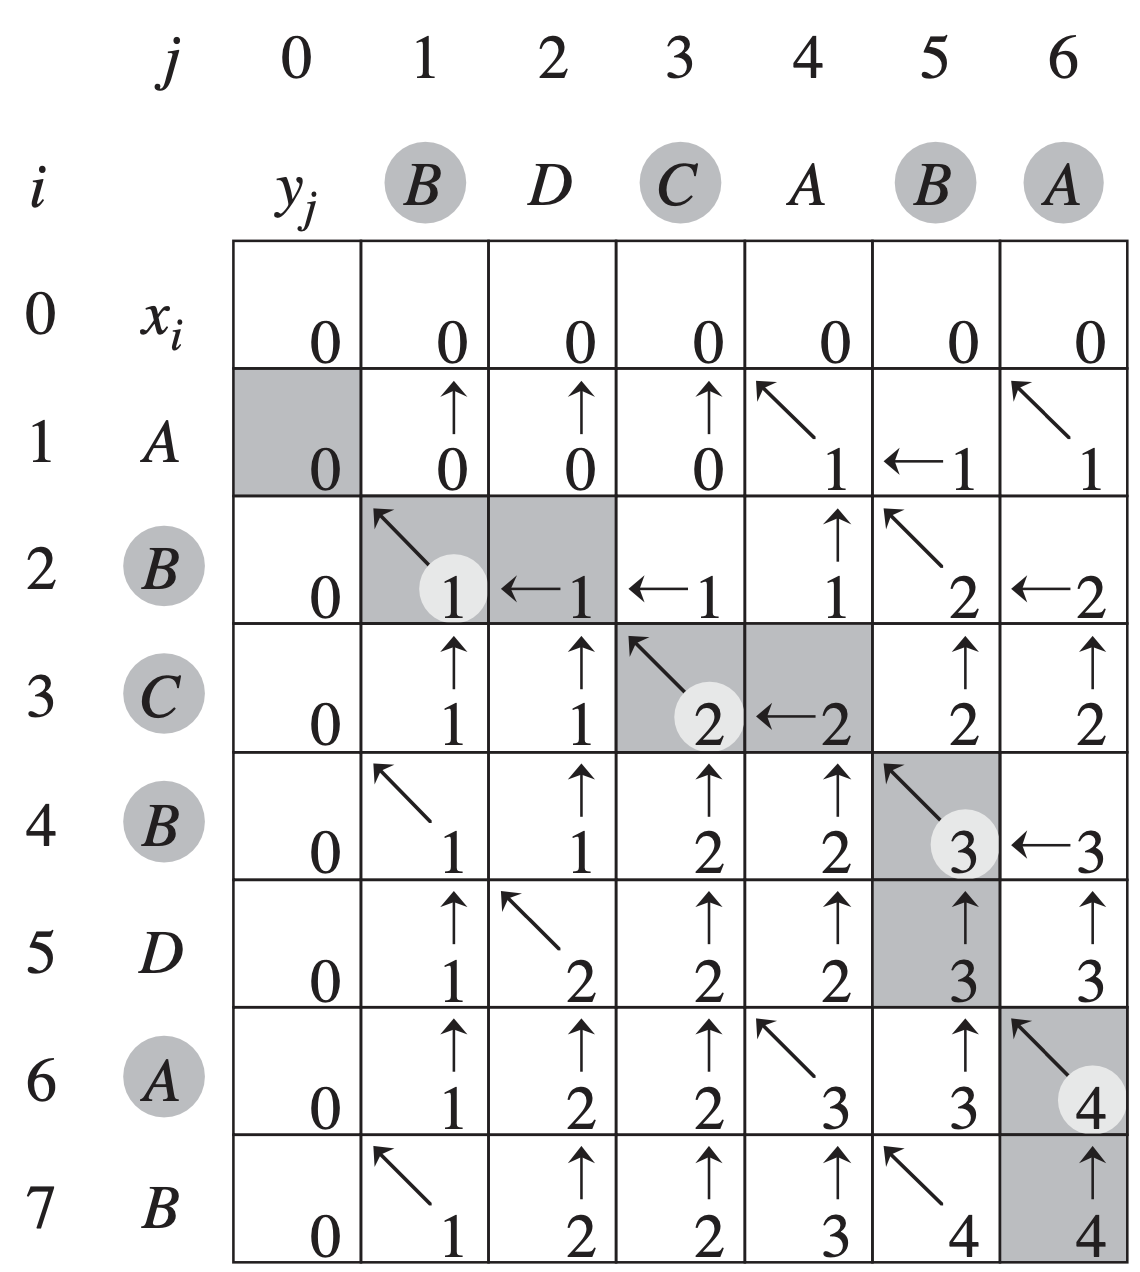
\includegraphics[width=.75\linewidth]{table}\\

\end{document}
